\documentclass[aspectratio=169,xcolor={svgnames}]{beamer}
% use this to generate the handout
% \documentclass[aspectratio=169,xcolor={svgnames},handout]{beamer}

\usepackage[utf8]{inputenc}

\usetheme[progressbar=frametitle,block=fill]{metropolis}
\usepackage{appendixnumberbeamer}

\title{Slide Examples}
\subtitle{\LaTeX Beamer}
\author{Wolfgang Hönig}
\date{October, 2023}

\begin{document}

  \frame[noframenumbering,plain]{\titlepage}

  \begin{frame}{Lists}

    \begin{itemize}
      \item Item1
      \item Item2
      \item Item3 with \alert{important} text
    \end{itemize}

  \end{frame}

  \begin{frame}{Enumerations}

    \begin{enumerate}
      \item Item1
      \item Item2
      \item Item3 with \alert{important} text
    \end{enumerate}

  \end{frame}

  \begin{frame}{Picture}
    
    \centering
    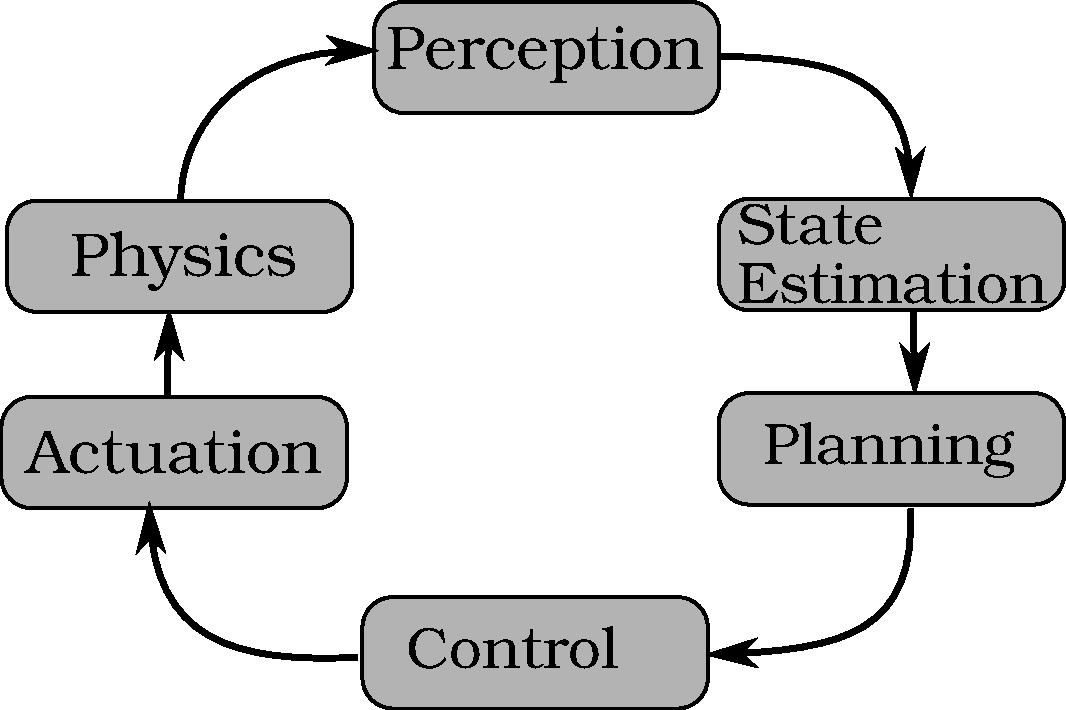
\includegraphics[width=0.6\textwidth]{images/robotics.pdf}

  \end{frame}

  \appendix

  \begin{frame}[standout]
    \inserttitle

    \begin{center}
      \resizebox{!}{0.4\textheight}{?}
    \end{center}

    \begin{columns}
      \begin{column}{0.55\textwidth}
        \begin{itemize}
        \item More Information:\\\url{https://whoenig.github.io}
        \end{itemize}
      \end{column}
      \begin{column}{0.45\textwidth}
        \begin{itemize}
        \item Contact:\\\href{mailto:hoenig@tu-berlin.de}{\texttt{hoenig@tu-berlin.de}}%\\
        \end{itemize}
      \end{column}
    \end{columns}
  \end{frame}

\end{document}
